% !TEX root = ../../../Masterthesis.tex

\chapter{Star Trek XI: Star Trek}\label{ch:st 11}

\section{Star Trek}

\begin{figure}[h!]
\center
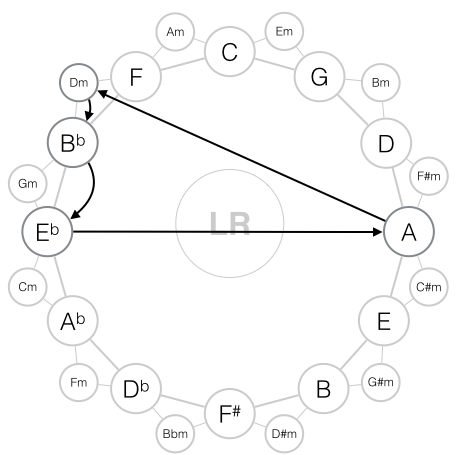
\includegraphics[width=0.7\linewidth]{ST11_star_trek_1}
	\caption{ST 11: Star Trek}
	\label{ST11_star_trek_1}
	%\setfloatalignment{b}
\end{figure}

\begin{marginfigure}
%\center
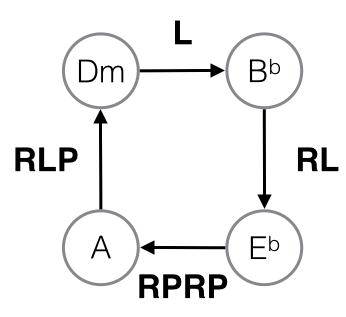
\includegraphics[width=\linewidth]{ST11_star_trek_1_1}
	\caption{ST 11: Star Trek: Transformational Cycle}
	\label{ST11_star_trek_1_1}
	%\setfloatalignment{b}
\end{marginfigure}

\noindent\newthought{Not unlike the} rest of the Star Trek franchise, Star Trek XI begins with a short overture, presenting the main tonality and mood of the coming score. The cue is quite clearly constructed in the circle of fifths, but honoring the ``space progression'' \ac{MTTP}. The progression mapped out in Dm follows: \(i-\flatx{VI}-\flatx{II}-V\). The sonority is soft but curious, with pads and soft strings supporting the melody. The melody is built upon a simple motif that transforms with the harmony.

With the main theme presented, Giacchino presents the second main theme used throughout\footnote{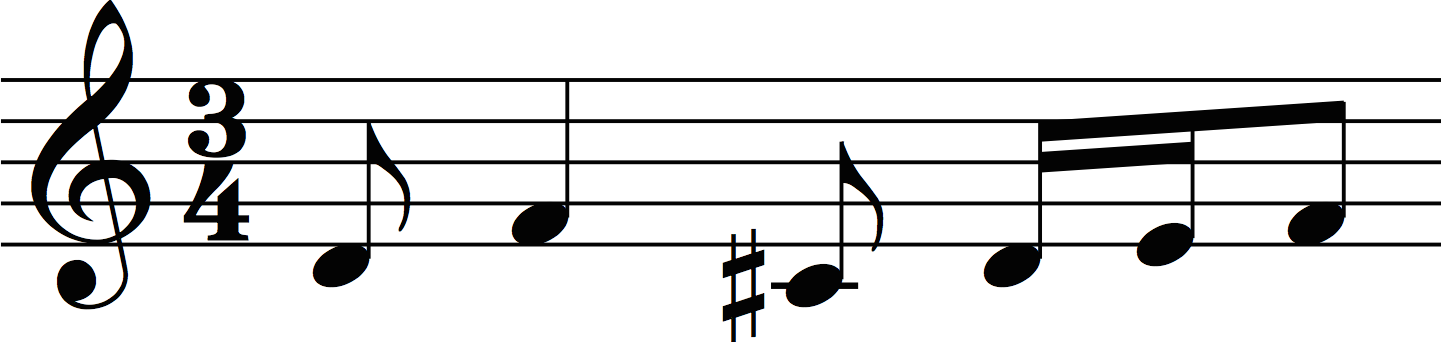
\includegraphics[width=\linewidth]{ST11_motif}}. 
%-----------------------------------------------------------------------------
% PDF
%-----------------------------------------------------------------------------
\clearpage
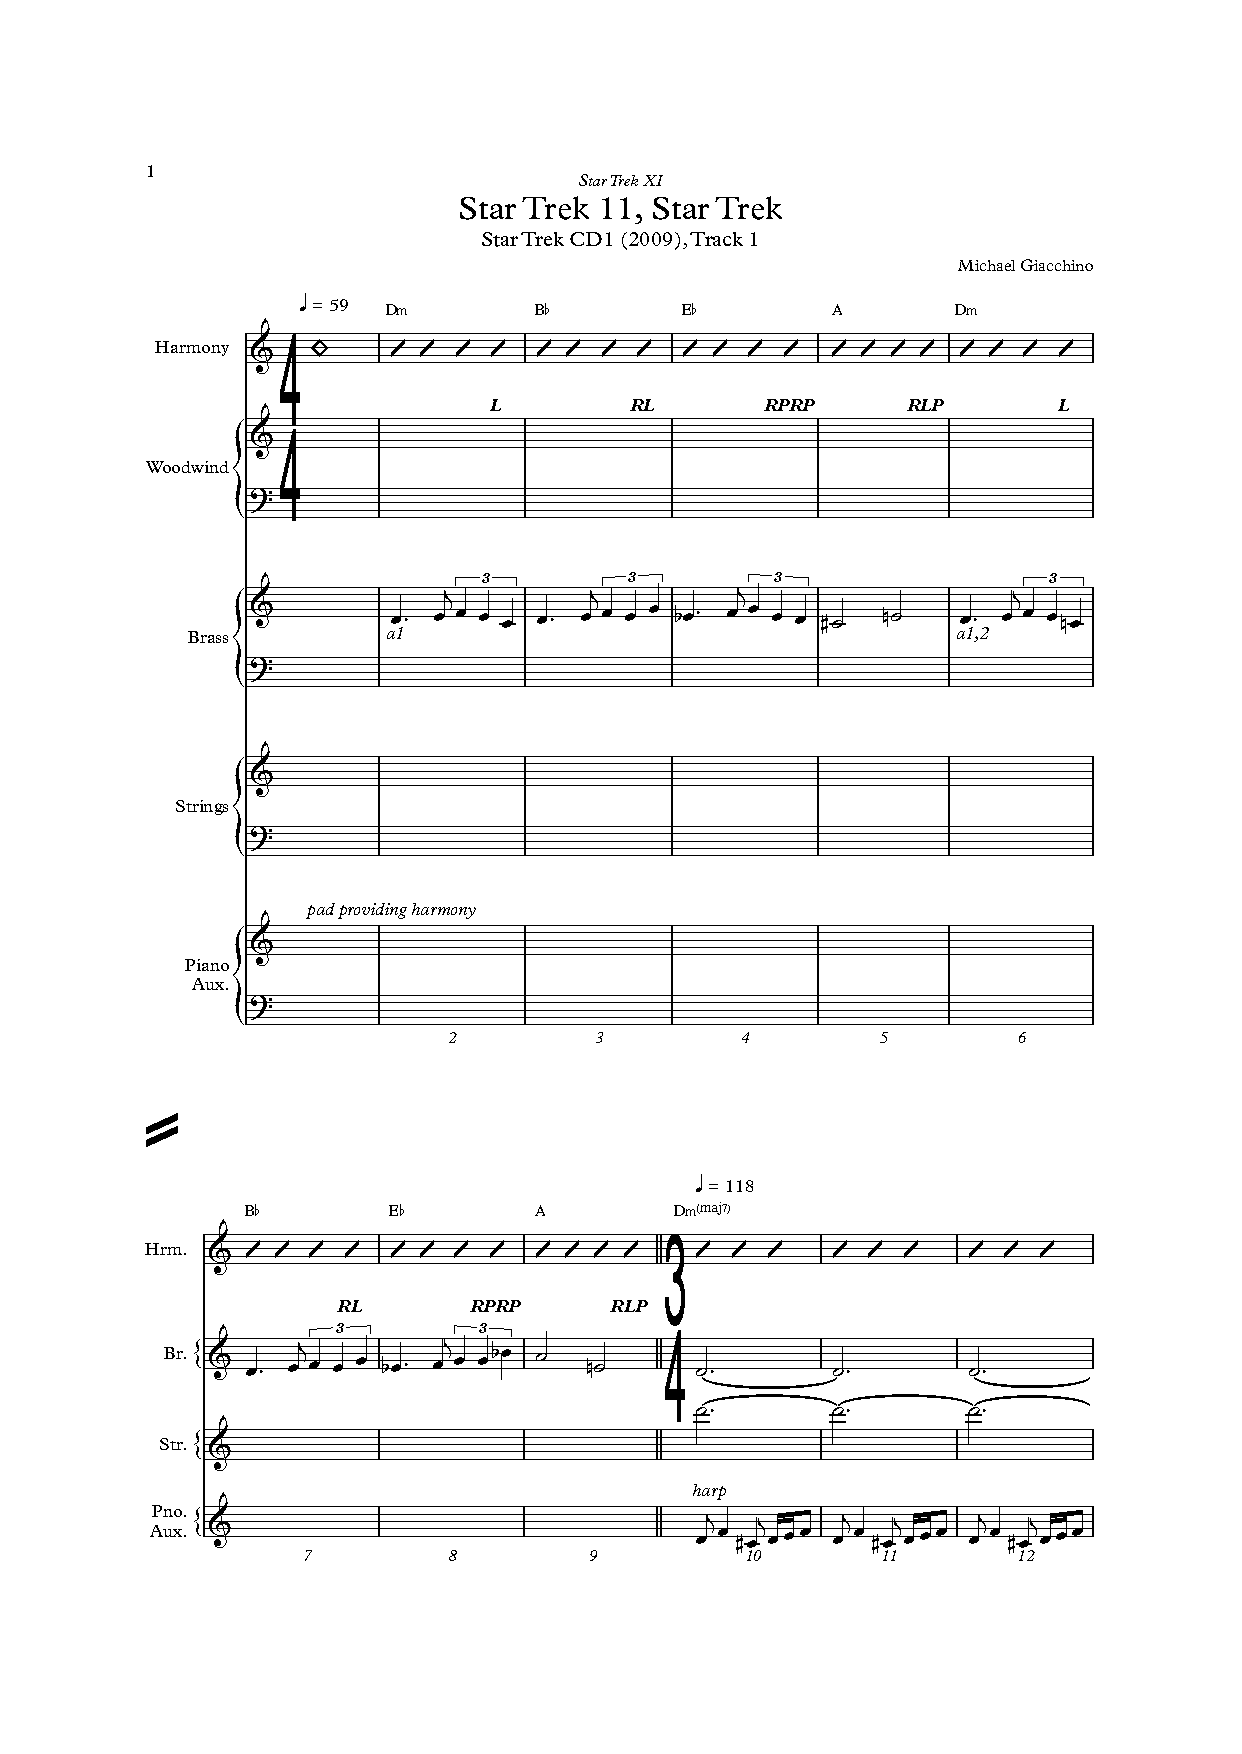
\includepdf[pages=-,pagecommand=\thispagestyle{fancy}]{pdf/ST11/ST_11_1_Star_Trek.pdf}

% Reviewed